\subsection{Theoretical Analysis}
In this section we present the model for the theoretical analysis of the bridge framework. 
We also present conjectures that we plan to prove if the grant is approved.
\subsection{Preliminaries}
\noindent
\textbf{Execution model.}
A ledger protocol $\Pi$ is a distributed protocol that offers
a \emph{read} and \emph{write} functionality.
The ledger protocol is accompanied by a \emph{validity language}
$\mathbb{V}_{\Pi}$ containing all possible transactions that are ``legal''
according to the protocol $\Pi$.
The
\emph{read} functionality returns a \emph{ledger} in $\mathbb{V}_{\Pi}^*$,
whereas the \emph{write} functionality accepts a ledger and a \emph{transaction} in $\mathbb{V}_\Pi$.
The \emph{ledger} is a finite sequence of pairs $(t, \tx)$ consisting
of an integer timestamp $t$ and a transaction $\tx$.

A particular protocol \emph{execution}
is one run of an environment $\mathcal{Z}_{\Pi,\mathcal{A}}$~\cite{FOCS:Canetti01} which simulates
the execution of $\Pi$ among multiple honest and adversarial parties. The adversarial
parties are controlled by one PPT adversary $\mathcal{A}$. The adversary and honest
parties are modelled as Interactive Turing Machines.
Out of the
$n_\Pi$ parties maintaining the ledger, $t_\Pi$ are corrupt and are controlled by the adversary
$\mathcal{A}$.

\noindent
\textbf{Networking.}
Time evolves in \emph{synchronous} lock-step \emph{rounds} denoted by the integers $1, 2,
\ldots$. All parties have perfectly synchronized clocks, as they know the current round number.
Messages which are broadcast by an honest party at a round $r$ are received by all
other honest parties at the beginning of the next round $r + 1$. The adversary
can reorder messages, potentially different for each honest party, and
inject different messages to the network tapes of different honest parties,
but cannot drop messages. We work in the \emph{client gossiping model}, where
a new message received by any honest party is rebroadcast to all other honest
parties; therefore, a party cannot identify the origin of a message. We assume there are no bandwidth constraints.
The total execution time is polynomial, and each (honest or adversarial)
party is bound to polynomial time per round.

\noindent
\textbf{Sequence notation.}
$x \in A$ denotes that either $x$ is an element of set $A$ or $x$
appears in the sequence $A$. We use $|A|$ for the length of the sequence $A$.
We write $A[i]$ for the $i$-th element of $A$ ($0$-based) and $A[-i]$ for the
$i$-th element of the inverse $A$ ($1$-based); the element $A[-1]$ is the last element of $A$.
We denote by $A[{i}{:}{j}]$ the subarray of $A$ starting from element $i$ (inclusive)
and ending in element $j$ exclusive. The notation $A[{:}j]$ means the sequence
from the beginning up to $j$, whereas $A[i{:}]$ means the sequence from $i$ till
the end.

\noindent
\textbf{Ledgers.}
We denote $\Ledger[\Pi][P][r]$ the result of executing the \emph{read} functionality by party $P$
operating in ledger protocol $\Pi$ at round $r$. % Therefore, the ledger $\Ledger[\Pi][P][r]$ of party $P$ at round $r$ is a sequence of transactions.
We will write
$a \in S$ for an element $a$ and a sequence $S$ if the element $a$ appears somewhere in
the sequence $S$. For a ledger $L$ we will also use the notation $\tx \in L$ to mean that
the transaction $\tx$ appears in $L$ with some timestamp, that is, there exists some $t \in \mathbb{N}$
such that $(t, \tx) \in L$. In all practical blockchain-based ledger protocols, the timestamp $t$
associated with a transaction will correspond to the timestamp recorded on the block in which the
transaction is confirmed. As such, timestamps will all be in the past and non-decreasing.

A ledger protocol is \emph{safe} if the view of different honest parties is consistent.

\begin{definition}[Persistence]
  A ledger protocol $\Pi$ is \emph{persistent} during $I$ if for all honest parties $P_1, P_2$ at rounds
  $r_1, r_2 \in I$, with $r_1 < r_2$,
  we have that $\Ledger[\Pi][P_1][r_1] \preceq \Ledger[\Pi][P_2][r_2]$.
\end{definition}

A ledger protocol is \emph{live} if honest transactions make it to the ledger.

\begin{definition}[Liveness]
  A ledger protocol $\Pi$ is \emph{live} with liveness $u \in \mathbb{N}$ during $I$ if,
  for all honest parties $P_1, P_2$, whenever
  $P_1$ attempts to write a \emph{valid} transaction $\tx$ to the ledger at round $r \in I$,
  then for all $r' \in I$ with $r' \geq r + u$
  the transaction is included in $\Ledger[\Pi][P_2][r']$.
\end{definition}

\begin{definition}[Timeliness]
  A ledger protocol $\Pi$ is \emph{timely} with timeliness $\nu \in \mathbb{N}$ during $I$ if,
  for all honest parties $P$, and for all rounds $r$, it holds that:

  \begin{enumerate}
    \item $\Ledger[\Pi][P][r][-1]$ has a timestamp in the past, and
    \item $\Ledger[\Pi][P][r]$ has non-decreasing timestamps.
  \end{enumerate}

  Additionally, for all rounds $r \in I$, it holds that
  the timestamps recorded in $\Ledger[\Pi][P][r][|\Ledger[\Pi][P][r-1]|{:}]$
  are after $r - \nu$.
\end{definition}

Ledger security is defined as a ledger protocol that is both safe and live.

\begin{definition}[Security]
  A ledger protocol is \emph{secure} during $I$ with liveness $u$ if it is:

  \begin{enumerate}
    \item \emph{persistent} during $I$,
    \item \emph{live} with liveness $u$ during $I$, and
    \item \emph{timely} with timeliness $\tau$ during $I$.
  \end{enumerate}
\end{definition}

\noindent
\textbf{Bridges.}
A \emph{bridge} $\Lambda(\Pi_1, \Pi_2)$ is an interoperability protocol between two ledger protocols
$\Pi_1$ and $\Pi_2$. The execution is defined by a \emph{shared} environment $\mathcal{Z}$ between $\Pi_1$
and $\Pi_2$, but each of $\Pi_1$ and $\Pi_2$ are simulated internally by the environment as before.
The purpose of the bridge is to relay events or information that take place on the source
side to the destination side. Without loss of generality, we consider $\Pi_1$ to be the \emph{source},
and $\Pi_2$ to be the \emph{destination}. If the bridge is bidirectional, our statements can be
applied in both directions. For our purposes, the purpose is to move value from one side to
the other.

A population of $n$ nodes, among which at most $t$ are adversarial, are
responsible for operating the bridge. The bridge transmits certain transactions
of interest from $\Pi_1$ to $\Pi_2$. These are \emph{cross-chain} transactions
and are defined by a function $\phi$ which accompanies the bridge protocol.

\begin{definition}[Cross-chain transaction]
  Let $\phi$ be an efficiently computable and invertible one-to-one
  injection $V_{\Pi_1} \longrightarrow V_{\Pi_2} \cup \{ \bot \}$.
  A transaction $\tx$ on the source side is a \emph{cross-chain} transaction if
  $\phi(\tx) \neq \bot$.
\end{definition}

A bridge is secure (Definition~\ref{def:bridge-security}) if it guarantees two fundamental properties:
safety (Definition~\ref{def:bridge-safety}) and liveness (Definition~\ref{def:bridge-liveness}).

\begin{definition}[Bridge Safety]\label{def:bridge-safety}
  A bridge protocol $\Lambda(\Pi_1, \Pi_2)$ is \emph{safe} with \emph{safety} $u_s \in \mathbb{N}$
  during $I$ if, for all honest parties $P_1$ of $\Pi_1$ and $P_2$ of $\Pi_2$ and for all rounds
  $r_1, r_2 \in I$ with $r_2 \geq r_1 + u_s$ we have that, whenever $(t, \tx) \in \Ledger[\Pi_2][P_2][r_1]$
  with $t \in I$ and $\phi^{-1}(\tx) \neq \bot$, then
  $\phi^{-1}(\tx) \in \Ledger[\Pi_1][P_1][r_2]$.
\end{definition}

\begin{figure}
    \center
    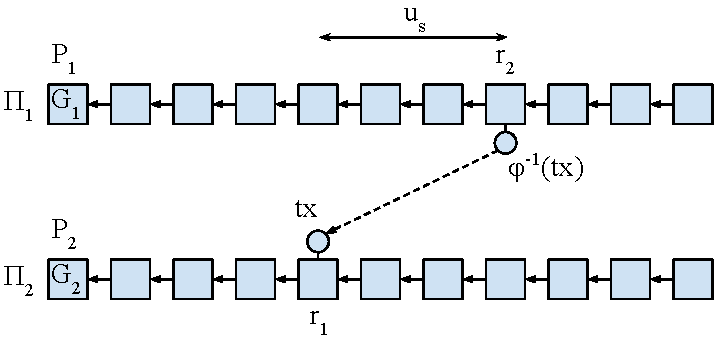
\includegraphics[width=0.8\columnwidth]{figures/bridge-safety.pdf}
    \caption{Bridge safety}
    \label{fig:bridge-safety}
\end{figure}

\begin{definition}[Bridge Liveness]\label{def:bridge-liveness}
  A bridge protocol $\Lambda(\Pi_1, \Pi_2)$ is \emph{live} with \emph{liveness} $u_\ell \in \mathbb{N}$
  during $I$ if, for all honest parties $P_1$ of $\Pi_1$ and $P_2$ of $\Pi_2$ and for all rounds
  $r_1, r_2 \in I$ with $r_2 \geq r_1 + u_\ell$ we have that, whenever $(t, \tx) \in \Ledger[\Pi_1][P_1][r_1]$
  with $t \in I$ and $\phi(\tx) \neq \bot$, then $\phi(\tx) \in \Ledger[\Pi_2][P_2][r_2]$.
\end{definition}

\begin{figure}
    \center
    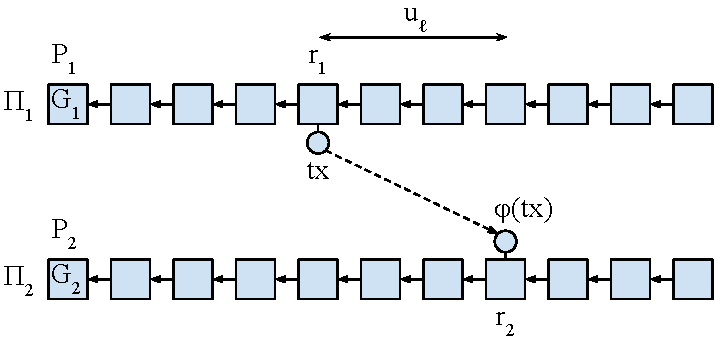
\includegraphics[width=0.8\columnwidth]{figures/bridge-liveness.pdf}
    \caption{Bridge liveness}
    \label{fig:bridge-liveness}
\end{figure}

\begin{definition}[Bridge Security]\label{def:bridge-security}
  A bridge $\Lambda$ is \emph{secure} with safety $u_s \in \mathbb{N}$ and
  liveness $u_\ell \in \mathbb{N}$ during $I$ if it is safe with safety $u_s$ during $I$
  and live with liveness $u_\ell$ during $I$.
\end{definition}

% - safety under dishonest majority in axelar network
% - healing
% - incentives
